\chapter{Passive Network Monitoring}
\label{chap-livenet}


\section{Introduction}
\label{sec-livenet-intro}

As sensor networks become more sophisticated and larger in scale,
better tools are needed to study their behavior in live deployment 
settings. Understanding the complexities of network dynamics, such 
as the ability of a routing protocol to react to node failure, 
or an application's reaction to varying external stimuli,
is currently very challenging. Simulators~\cite{tossim,avrora} and 
testbeds~\cite{motelab,mirage} offer the
opportunity to understand sensor applications in controlled settings.
However, no good tools exist to observe and monitor a sensor 
network deployment {\em in situ}.

In many cases, it is difficult or impossible to add new
instrumentation into a deployed sensor network. Depending on the
circumstances, reprogramming nodes may be impossible or inadvisable
(for example, due to downtime or risk of breaking an existing system). 
Also, adding debugging code adds overhead and consumes memory, CPU, and
network resources. Additionally, the instrumentation code itself 
may alter the behavior of the deployed network in subtle ways.
Using a wired back-channel (as is commonly used in testbeds) 
is not possible in deployments where nodes may be mobile or
located in remote environments.

In this chapter, we describe {\em LiveNet}, a set of tools and techniques
for recording and reconstructing the complex dynamics of live sensor network
deployments. LiveNet is based on the use of passive monitoring of radio
packets observed from one or more {\em sniffers} that are co-deployed with the
network. Sniffer nodes can be
either temporary or permanent, fixed or mobile, and 
wired or untethered. 
Sniffers record traces of all packet activity observed on the
radio channel.
Traces from multiple sniffers are merged into a single
trace to provide a global picture of the network's behavior. The
merged trace is then subject to a series of analyses to study
application behavior, data rates, network topology, and routing protocol 
dynamics. 

Using passive monitoring to understand a sensor network's behavior
raises a number of unique challenges. First, we are concerned with the
coverage of the LiveNet sniffer infrastructure in terms of total
number of packets observed by the system. Second, the merging process 
can be affected by incomplete packet traces and lack of time
synchronization across sniffers. We make use of an approach similar to
Jigsaw~\cite{jigsaw} and Wit~\cite{wit} to merge multiple traces, with
modifications specific to the use of IEEE 802.15.4 networks. Third,
understanding global network behavior requires extracting aggregate
information from the detailed traces. We describe a series of
analyses, including a novel {\em path inference} algorithm 
that derives routing paths based on incomplete packet traces.


We evaluate the use of LiveNet by performing an extensive validation 
of LiveNet using measurements on MoteLab.
Our results show that deploying a LiveNet infrastructure along with an
existing sensor network can yield a great deal of valuable information
on the network's behavior without requiring additional instrumentation
or changes to the sensor network code. Our packet merging process and 
trace analyses yield an accurate picture of the network's operation.
Finally, we show that our path inference algorithm correctly determines 
the routing path used without explicit information from the routing
protocol stack itself. 



\section{LiveNet architecture}
\label{sec-livenet-arch}

\begin{figure}[t]
\begin{center}
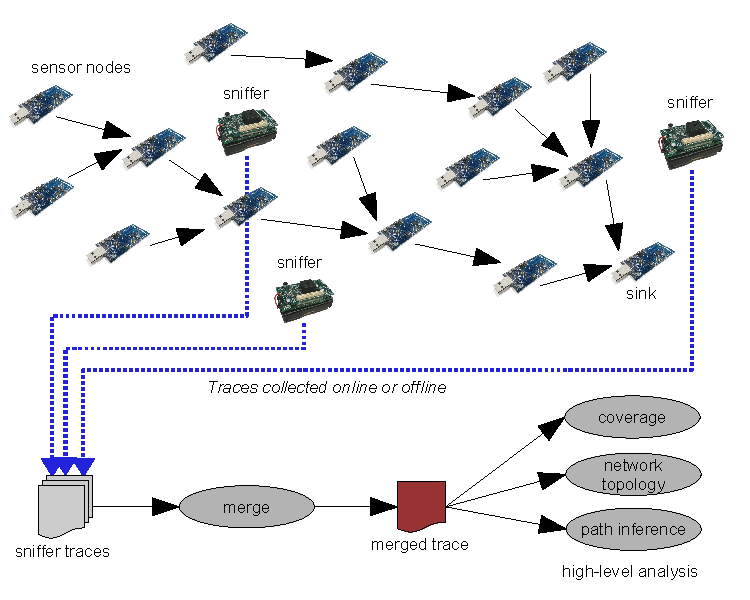
\includegraphics[width=0.6\hsize]{./resources/livenet-sensys07/figs/arch.pdf}
\end{center}
\caption{\small {\bf Overview of the LiveNet architecture.}}
\label{fig-arch}
\end{figure}

LiveNet consists of three main components: a {\em sniffer
infrastructure} for passive monitoring and logging of radio packets; 
a {\em merging process} that normalizes multiple sniffer logs and 
combines them into a single trace; and a set of {\em analyses} 
that make use of the combined trace. 
While packet capture is performed in real time, merging and analysis
of the traces is performed offline due to high storage and
computational requirements. While providing real-time analysis
of traffic captured by LiveNet would be useful in certain situations,
we believe that offline trace merging and analysis meets many of the
needs of users wishing to debug and analyze a network deployment.

\subsection{Sniffer infrastructure}

The core of the LiveNet infrastructure is a set of passive network
sniffers that capture packets and log them for later analysis.
Conceptually the sniffer is very simple, consisting of a sensor node
either logging packets to local flash or over its serial port to an
attached host. However, certain factors
must be taken into account to achieve the desired level of fidelity in
the recorded packet trace.

First of all, sniffers must timestamp packets as they are received 
by the radio, to facilitate later timing-based analysis as well as 
merging of traces. This timestamping can be performed at different
levels depending on the desired degree of accuracy. Stamping packets
as they are received by the mote's radio stack offers the lowest
latency between packet reception and timestamp capture. Timestamping
as the packet is received by the sniffer application may suffer
delays due to packet processing (e.g., posting the packet receive
task in TinyOS). Timestamping at the host attached to the sniffer, 
if any, involves the highest latency as packets must be transferred
over the serial port prior to stamping.

Our prototype uses hardware timers provided by the CPU (as 
appropriate for each mote platform) to timestamp packets in the 
{\em ReceiveMsg.receive()} interface; on the MSP430 this is a 32~kHz timer. 
Hooking into the CC2420 radio stack would offer lower latency for
timestamping, however, none of the analyses that we perform required
this higher degree of accuracy.

We assume that all sensor nodes are sharing
the same radio channel and that sniffers are tuned to the same
channel as the network. In cases where frequency hopping is used,
sniffers need to {\em scan} multiple channels or match the
frequency-hopping schedule of the sensor nodes. However, frequency hopping 
is not common in 802.15.4-based sensor networks deployed to date. 

In our current prototype, each received radio packet is wrapped in an
envelope and enqueued for transmission over the mote's serial port.
The envelope contains the timestamp, ID of the sniffer node, and
original radio packet contents.
A host attached to the mote is responsible for logging the packet.
This host could be a laptop or PC, or a USB-to-Ethernet bridge such as
the TMote Connect. The host logs each packet in a raw format as it is
received over the serial port to a file or database.

{\bf Deployment scenarios:}
We envision a range of deployment options for LiveNet
sniffers. Sniffers can be installed either temporarily, 
during initial deployment and debugging, or permanently, 
in order to provide an unobtrusive monitoring framework. Temporary
sniffers could log packets to flash for manual retrieval, while
permanent sniffers would typically require a back-channel for
delivering packet logs. Another scenario might involve one or more
{\em mobile} sniffers, each carried by an individual around the sensor
network deployment site. This would be particularly useful for
capturing packets to debug a performance problem without disturbing 
the network configuration.  

\subsection{Merging process}
\label{sec-livenet-merging}

Given a set of sniffer traces $\{ S_1 \ldots S_k \}$, a core problem 
is how to
combine these traces into a temporally-ordered log that represents the
union of the packets observed by each sniffer, offering a global view
of network activity. 

Several challenges arise when merging multiple sniffer traces.
First, each trace will contain only a subset of the overall set of
packets received, so it is important to interleave multiple traces
while preserving the correct packet order. Second, we do not assume
that sniffers are time synchronized, so two sniffers logging the same
packet will use different timestamps. Therefore, we must first {\em
normalize} the timebase used across each trace, in effect performing
{\em post hoc} time synchronization. Third, link-level retransmission
of a packet can cause multiple copies of the same packet contents to
appear in each sniffer trace, making it difficult to
disambiguate individual packet transmissions from each other.

Our approach to trace merging is inspired by Jigsaw~\cite{jigsaw} 
and Wit~\cite{wit}, which perform merging of multiple 802.11 packet 
traces. Although there are similarities between these systems and 
LiveNet, as described in Section~\ref{sec-livenet-background}, there are 
important differences owing to the nature of sensor networks, in 
particular multihop traffic. We briefly describe the process here,
referring the reader to~\cite{jigsaw,wit} for additional background.

\subsubsection{Timing normalization}

The first step is to {\em time correct} each of the sniffer traces so
that a unique packet logged in multiple traces will have a (near)
identical timestamp. We choose an arbitrary sniffer trace $S_0$ as
a timebase reference and map packets in all other traces to this timebase.
Let $t_p^i$ represent the timestamp associated with packet 
$p$ logged in trace $S_i$. 
Our goal is to assign a timestamp $\hat{t}_p^i$ such that $\hat{t}_p^i \approx
t_p^0$ (assuming that $p$ was logged in sniffer trace $S_0$).
Note that due to slight timing jitter between sniffers,
even after time correction, not all instances of $p$ logged in all
traces will have an identical corrected timestamp $\hat{t}_p^i$.

To accomplish this, we calculate a {\em time mapping} 
$\Delta_i$ such that $\hat{t}_p^i = t_p^0 + \Delta_i$. The time
mapping represents a constant time offset between packets logged 
in $S_0$ and $S_i$. This accounts for a constant time shift between
two sniffers. Rather than directly account for clock skew, we 
partition the sniffer trace into multiple {\em intervals} and
compute $\Delta_i$ separately for each interval. The duration of
the interval is selected so that any accumulated clock skew will not
introduce large errors in the corrected timestamps; we set the
interval length to 1~hour in our prototype.


In the case where sniffers $S_0$ and $S_i$ both log the same packet
$p$, computing the time mapping $\Delta_i$ is straightforward:
$\Delta_i = t_p^i - t_p^0$. However, depending on the physical
placement of sniffers, it is likely that $S_i$ and $S_0$ may not
overhear any packets in common. In general, we compute the time
mapping using a {\em time offset graph} $G(V,E)$ where each vertex 
in $V$ represents a sniffer, and edges in $E$ represent the time
offset between two sniffers that log at least one packet $p$ in
common. The weight of each edge $E(S_i,S_j) = \Delta_{i,j}$. 
The time offset $\Delta_i = \Delta_{i,0}$ is computed by taking 
the shortest weighted path in the time graph from $S_i$ to $S_0$.

The time mapping algorithm proceeds as follows. Each trace is
scanned one packet at a time and a hash of the contents of the packet 
$h(p)$ is computed. We record the tuple $(S_i, t_p^i)$ in a hashtable
with key $h(p)$. If the same packet is recorded in multiple traces, 
these entries will match the same hash bucket. When this occurs, we
add two edges to the time graph with weights $\Delta_{i,j}$ and
$\Delta_{j,i}$ respectively. If $\Delta_i$ or $\Delta_j$ are unknown,
we test for a shortest path to $S_0$ in the time graph to compute the
missing value. The algorithm terminates when either $\Delta_i$
has been computed for all sniffers $i$, or all packets from all
sniffer logs have been read. It is possible that after this process 
we cannot compute $\Delta_i$ for certain sniffers, at which 
point those sniffers are excluded from further analysis.

To avoid ambiguity in computing the time mapping, we only consider 
{\em unique} packets $p$ in the sniffer traces, that is, packets that 
will not be logged multiple times by the same sniffer with 
multiple timestamps. For example, when using link-layer ARQ, a packet
might be transmitted multiple times with an identical payload,
leading to an ambiguity about which instances of $p$ correspond to 
each other in different sniffer traces. 
For timebase construction, we only consider packets that are expected
to be unique in a given sniffer trace: for example, any packet with a
unique sequence number assigned by the transmitting node.
Rollover in the sequence numbers (for example, if only an
8-bit sequence number field is used) is easily handled by
first pre-scanning the sniffer traces and assigning a {\em
pseudo-sequence number} that will not roll over (e.g., using a 64-bit
value).

\subsubsection{Progressive trace merging}

The second step is to merge the sniffer traces and write out a single
combined trace. Because individual traces can be very large, it is
impractical to read each trace into memory, perform a merge, and
write out the result. For example, traces from the disaster drill
deployment (described in Section~\ref{sec-livenet-deployment}) were up to 
37~MB in size for a log covering less than 90~minutes of trace data.
This requires that we perform a {\em progressive} merging of
individual traces, writing out the merged results on the fly. 

Our algorithm operates by alternating between two phases: 
{\em scanning} and {\em emitting}. 
In the scanning phase, we scan packets from each trace 
$S_i$. The packet contents are read and the time
mapping $\Delta_i$ applied to each packet. Packets are inserted
into a priority queue sorted by timestamp. If a packet with
identical contents (as determined by the hash function $h(p)$) is
already in the priority queue, it is {\em merged} into a single
packet, retaining information about the set of traces in which the
packet was identified and the maximum time spread 
$\Delta t = \max_{\forall S_i,S_j} (\|t_p^i - t_p^j\|)$ between 
any two instances of the packet in the priority queue. We continue
scanning packets from the same source $S_i$ until $\hat{t}_p^i$ 
is greater than or equal to the highest timestamp of packets already 
in the priority queue.


Once we have scanned all traces $\{S_1 \ldots S_k\}$ in this
manner, we begin an emitting phase. We iterate over the priority
queue (ordered by the time-corrected timestamp) and emit each packet
$p$ into the merged trace. (Recall that $p$ may have been merged with 
identical packets from other traces during the scanning phase.) The
emitting phase continues until one of two conditions occurs: (1) The
packet $p$ popped from the priority queue has a time offset of 
$\sigma$~sec greater than the previously emitted packet, or (2) The
length of the priority queue (time offset between the first and last
packet) is less than $\eta$~sec. In the former case, we
withhold emitting the packet, place it back on the priority queue
and, return to the scanning phase. The idea is that if there is a
gap in the emitted packet stream, it may be necessary to scan more
packets in order to fill in the gap. In the latter case, we want to
keep the priority queue populated with enough packets to ensure that
merging will be successful across traces. 
If we have completed scanning all traces then we do not require this
latter condition to hold. 

Because the merging process operates in a progressive fashion, there
is some chance that a packet $p$ will be ``prematurely'' emitted, that
is, before all matching copies of $p$ across all traces have been
scanned. This will lead to a duplicate of $p$ in the merged trace. 
In general, it is impossible for us to ensure that we scan
all copies of a packet before emitting, unless we read all traces
into memory before emitting (effectively setting $\eta = \infty$).
In our implementation, we use $\sigma = \eta = 10$~sec in order to
bound memory usage. 
Removal of duplicates is easily corrected by running the merge 
a second time on the merged trace itself, which will cause 
any duplicates to be merged together.
In practice we find that our choice of parameters results in very few
duplicate packets.


\subsubsection{Handling duplicate transmissions} 

As stated earlier, multiple
transmissions of the same packet (say, due to link-layer ARQ) will
cause several copies of the same packet to appear in the sniffer
traces, and complicates the merging process. Denote
$\mathrm{dups}_i(p)$ as the number of duplicates of packet $p$ seen
in trace $S_i$. For example, consider traces $S_1$ with 
$\mathrm{dups}_1(p) = 4$ and $S_2$ with $\mathrm{dups}_2(p) = 2$.
The question is how many copies of $p$ should appear in the merged
trace $S_1 \cup S_2$.

Without any other information to uniquely
identify the multiple copies of $p$, we opt to adhere to the lower
bound, $d^\star = max_i (\mathrm{dups}_i(p))$. We know that {\em at least} 
this many copies of $p$ were transmitted, so this is a
conservative estimate. Taking the upper bound, 
$\sum_i \mathrm{dups}_i(p)$, assumes that there is no
overlap in the copies of $p$ observed across traces. 
Our merging process combines all copies of $p$ seen in the input
traces and attaches the value of $d^\star$ to the packet in the merged trace. 

Two pieces of information could be used to improve this estimate.
The TinyOS CC2420 radio stack includes the {\tt\verb+tos_dsn+} field in
each packet, which is incremented for each individual packet
transmission. Taking $d' = \max(\mathtt{tos\_dsn}_p) - 
\min(\mathtt{tos\_dsn}_p)$
improves upon our lower bound. Unfortunately, 
the MicaZ implementation of the TinyOS serial stack rewrites 
packets into an older format that does not include this field, so
this information is not available when using a MicaZ as a
sniffer.\footnote{Although this could be fixed in the TinyOS code,
our sniffer traces from the live disaster drill used the original
MicaZ serial stack and therefore are lacking the {\tt tos\_dsn} field.}
One can also improve the estimate of $d^\star$ by estimating the 
{\em overlap} between two sniffers $S_1$ and $S_2$ based on the
fraction of matching (unique) packets in both traces. 
We leave exploration of these ideas to future work.


\section{Trace Analysis}
\label{sec-livenet-analysis}

A wide range of analyses can be performed on the merged LiveNet 
packet trace. In this section, we describe a range of analysis
algorithms for reconstructing a sensor network's behavior. Several of
these algorithms are generic and can be applied to essentially any
type of traffic, while other analyses use application-specific
knowledge. 

\subsection{Coverage analysis}

The most basic analysis algorithm attempts to estimate the {\em
coverage} of the LiveNet sniffer infrastructure, by computing the
fraction of packets actually transmitted by the network that were
captured in the merged packet trace. Coverage can also be computed on
a per-sniffer basis, which is useful for determining whether a given
sniffer is well-placed. 

Let us define $C_i(n)$ as the coverage of sniffer $S_i$ for packets
transmitted by node $n$. Over a representative time interval $t$, we can
compute 
\[ 
C_i(n) = \frac{\sum_t \mathrm{packets\ from\ } n \mathrm{\ received\ by\ } S_i}{\sum_t
\mathrm{packets\ transmitted\ by\ } n}
\]
Likewise, $C(n)$ can be computed for the merged trace $\cup_i S_i$.
This calculation requires an estimate of the number of packets
actually transmitted by each node $n$ during the time interval.
This information can be determined in several ways: for example,
using packet-level sequence numbers, or knowledge of the application
transmission behavior (e.g., if the application transmits a periodic
beacon packet). 

This analysis assumes that packet loss from nodes $n$ to sniffers
$S_i$ is uniform and does not depend on the contents of the packets.
Note that this assumption might not be valid, for example, if longer
packets are more likely to experience interference or path loss.

\subsection{Overall traffic rate and hotspot analysis}


Another basic analysis is to compute the overall amount of traffic
generated by each node in the network, as well as to determine
``hotspots'' based on which nodes appear to be the source of, or
destination of, more packets than others. Given the merged trace,
we can start by counting the total number of packets originating from
or destined to a given node $n$. Because LiveNet may not observe all 
actual transmissions, we would like to {\em infer} the existence of other
packets. For example, if each transmission carries a unique sequence
number we can infer missing packets by looking for gaps in the
sequence number space. Coupled with topology inference 
(Section~\ref{sec-livenet-topology}), one can also determine which nodes 
were likely to have received broadcast packets, which do not 
indicate their destination explicitly.

\subsection{Network connectivity}
\label{sec-livenet-topology}


Reconstructing radio connectivity between nodes is seemingly straightforward:
for each packet from node $a$ to $b$, we record an edge $a
\rightarrow b$ in the connectivity graph. However, this approach may
not reconstruct the {\em complete} topology, since two nodes $a$ and
$b$ within radio range may choose not to communicate directly, 
depending on the routing protocol in use. We make use of two
approaches. First, if one assumes that connectivity is symmetric, 
an edge $b \rightarrow a$ can be recorded alongside $a \rightarrow b$.
Although asymmetric links are common in sensor 
networks~\cite{scale}, our goal is only to establish
whether two nodes are potential neighbors.

The second method is to inspect routing control packets. For example, 
several routing protocols, such as TinyOS' {\tt MultihopLQI}, 
periodically transmit their {\em neighbor table} containing
information on which nodes are considered neighbors, sometimes 
along with link quality estimates. These packets can be used
to reconstruct the network connectivity from the sniffer traces. Note
that this information is generally not available to a base station, which 
would only overhear control packets within a single radio hop.

\subsection{Routing path inference}
\label{sec-livenet-path-inference}

\begin{figure}
\begin{center}
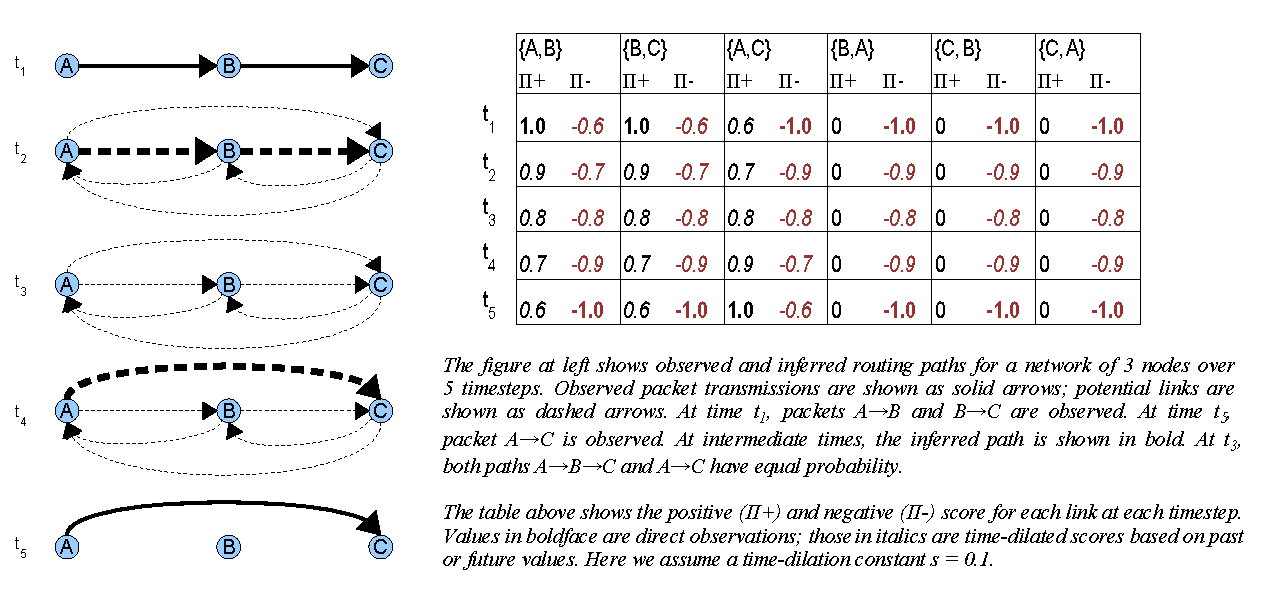
\includegraphics[width=0.9\hsize]{./resources/livenet-sensys07/figs/pathinference/path-example.pdf}
\caption{{\small\bf Path inference example.}}
\label{fig-pathinference-example}
\end{center}
\end{figure}

One of the more interesting analyses involves reconstructing
the routing path taken by a packet traveling from a source node $s$
to a destination $d$. The simplest case involves protocols that use
source-path routing, in which case the complete routing path is
contained within the first transmission of a packet from the
originating node. 


In most sensor network routing protocols, however, the
routing state must be inferred by observing packet transmissions as
packets travel from source to destination.
However, because the merged packet trace may not contain every routing 
hop, there is some ambiguity in the routing path that is
actually taken by a message. In addition, the routing path may evolve
over time. As a worst case, we assume that the route can change between 
any two subsequent transmissions from the source node $s$. 
Our goal of our path inference algorithm is to determine the {\em most
probable} routing path $P(s,d,t) = ( s, n_1, n_2, ... n_k, d )$ 
at a given time $t$ based on a possibly incomplete trace.


We begin by quantizing time into fixed-sized windows;
in our implementation the window size is set to 1~sec.
For each possible routing hop $a \rightarrow b$, we maintain a 
{\em score} $\Pi(a,b,t)$ that represents the likelihood of the hop
being part of the routing path during the window containing $t$.
$\Pi(a,b,t)$ is calculated using two values for each link:
a {\em positive score} $\Pi^+(a,b,t)$ and a {\em negative score}
$\Pi^-(a,b,t)$. The positive score represents any positive information
that a link may be present in the routing path, based on an
observation (possibly at a time in the past or future) that a message was
transmitted from $a$ to $b$. The negative score represents negative
information for links that are {\em excluded} from the routing path
due to the presence of other, conflicting links, as described below.
The probability of a link being part of the routing path 
is computed as a combination of the positive and negative scores, 
as described below.

Figure~\ref{fig-pathinference-example} shows our algorithm at work 
on a simple example.  We begin by initializing
$\Pi^+(a,b,t) = \Pi^-(a,b,t) = 0$ for all values of $a$, $b$, and $t$.
The merged packet trace is scanned, and for each packet transmission 
from $a$ to $b$, we set $\Pi^+(a,b,t) = 1$. For each {\em conflicting
link} $a' \rightarrow b'$, we set $\Pi^-(a',b',t) = -1$.
A link conflicts with $a \rightarrow b$ if it shares one endpoint in
common (i.e., $a = a'$ or $b = b'$); $b \rightarrow a$ is conflicted
by definition as well.

Once the scan is complete, we have a sparse matrix representing the
values of $\Pi^+$ and $\Pi^-$ that correspond to observed packet
transmissions. However, there are potentially many gaps in the packet
trace and we must assign values for the positive and negative scores
for times when no transmission on a link is observed. Our approach is to {\em
time dilate} the scores, in effect assigning ``degraded'' scores
to those times before and after each observation. 

Given a time $t$ for which no value has been assigned for $\Pi^+(a,b,t)$, 
we look for the previous and next time windows $t_f = t + \delta_f$ and
$t_b = t - \delta_b$ that have concrete observations 
$\Pi^+(a,b,t_f) = \Pi^+(a,b,t_b) = 1$. We then set:
\begin{eqnarray*}
\Pi^+(a,b,t) & =  & \max( \max(0, \Pi^+(a,b,t_f) - s \cdot \delta_f), \\
             &    & \max(0, \Pi^+(a,b,t_b) - s \cdot \delta_b))
\end{eqnarray*}
That is, we take the maximum value of $\Pi^+$ time-dilated backwards
from $t_f$ or forwards from $t_b$, capping the value to $\geq 0$.
Here, $s$ is a scaling constant that determines how quickly the score
degrades per unit time. 
Similarly, we fill in values for missing $\Pi^-(a,b,t)$ values, also
capping them to be $\leq 0$. In our implementation we set $s = 0.1$.

Once we have filled in all cells of the matrix for all links and all
time windows, the next step is to compute the final link score 
$\Pi(a,b,t)$:
\[
\Pi(a,b,t) = \left\{ \begin{array}{ll}
  \Pi^+(a,b,t) & \mbox{if $\Pi^+(a,b,t) \geq |\Pi^-(a,b,t)|$} \\
  \Pi^-(a,b,t) & \mbox{otherwise}
  \end{array}\right. 
\]
That is, the score is assigned to either the positive or negative
score, depending on which has the greater absolute value. Note that
for links for which we have no information, $\Pi(a,b,t) = 0$. 

We now have a complete matrix representing the score for each link at
each time window. The final step is to compute the most likely routing
path at each moment in time. For this, we take the acyclic path that has the
highest {\em average} score over the route, namely:
\[
P^\star(s,d,t) = \arg\max_{\forall P(s,d,t)} 
\frac{\sum_{l=\{n1,n2\} \in P(s,d,t)} \Pi(n_1, n_2, t)}{| P(s,d,t) |}
\]
The choice of this metric has several implications. First, links
for which we have no information ($\Pi(a,b,t) = 0$) diminish the
average score over the path. Therefore, all else being equal, 
our algorithm will prefer shorter paths over longer ones. 
For example, consider a linear path with a ``gap'' between two nodes 
for which no observation is ever made: $(s, n_1, \ldots ? \ldots, n_2, d)$. 
In this case, our algorithm will fill in the gap with the direct hop 
$n_1 \rightarrow n_2$ since that choice maximizes the average score
over any other path with more than one hop bridging the gap.

Second, note that the most likely path $P^\star$ may not be unique; 
it is possible that many routes exist with the same average score.
In this case, we can use network connectivity information 
(Section~\ref{sec-livenet-topology}) to exclude links that are not likely to
exist in the route. However, we cannot guarantee that this algorithm
always converges on a unique solution for each time window.
 


\section{Implementation}
\label{sec-livenet-impl}


Our implementation of LiveNet consists of three components: the sniffer
infrastructure, trace merging code, and analysis algorithms. The
sniffers are implemented as a modified version of the TinyOS {\tt
TOSBase} application, with two important changes. First, the code is
modified to pass every packet received over the radio to the serial
port, regardless of destination address or AM group ID. 
Second, the sniffer takes a local timestamp (using the 
{\tt SysTime.getTime32()} call) on each packet reception, and prepends 
the timestamp to the packet header before passing it to the serial port. 


We observed various issues with this design that have not yet been
resolved. First, it appears that TMote Sky motes have a problem
streaming data at high rates to the serial port, causing packets to
be dropped by the sniffer. In our LiveNet deployment described below, 
a laptop connected to both a MicaZ and a TMote Sky sniffer 
recorded more than three times as many
packets from the MicaZ. This is possibly a problem with the MSP430
UART driver in TinyOS. Second, our design only records packets
received by the Active Messages layer in TinyOS. Ideally, we would
like to observe control packets, such as acknowledgments, as well as
packets that do not pass the AM layer CRC check. 


Our merging and analysis tools are implemented in Python, using a
Python back-end to the TinyOS {\em mig} tool to generate appropriate
classes for parsing the raw packet data. The merging code is 
657~lines of code (including all comments). The various analysis
tools comprise 3662~lines of code in total. A separate library 
(131~lines of code) is used for parsing and managing packet traces,
which is shared by all of the merging and analysis tools.



\section{Validation Study}
\label{sec-livenet-validation}

The goal of our validation study is the ascertain the accuracy of the
LiveNet approach to monitoring and reconstructing sensor network
behavior. For this purpose, we make use of a well-provisioned indoor
testbed, which allows us to study LiveNet in a controlled setting.
The testbed consists of 184~TMote Sky nodes
deployed over several floors of an office building, located mainly on
bookshelves in various offices and labs. During the experiments
between 120--130 nodes were active. Each node is connected to a
USB-Ethernet bridge for programming and access to the node's serial
port. For our validation, half of the nodes are used as sniffers and the
other half used to run various applications. Although such a sniffer
ratio is much larger than we would expect in a live deployment,
this allows us to study the effect of varying sniffer coverage.

\subsection{Sniffer reception rate}

\begin{figure}[t]
\begin{center}
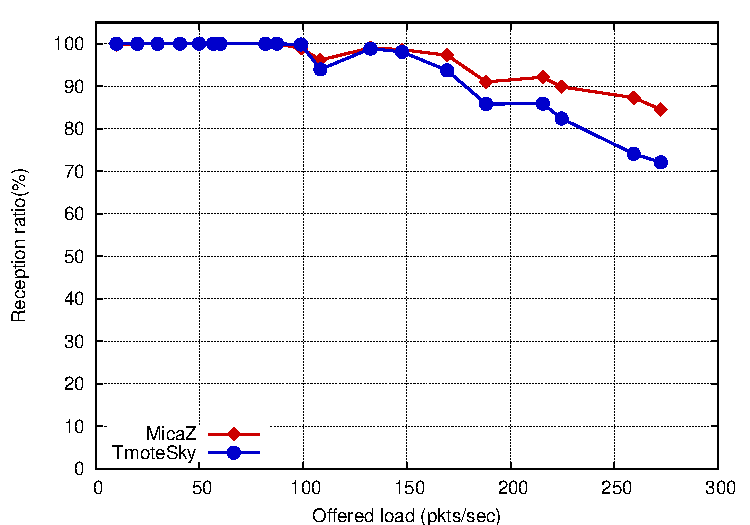
\includegraphics[width=0.6\hsize]{./resources/livenet-sensys07/figs/validation/rate-test/rate-test.pdf}
\end{center}
\caption{\small {\bf Sniffer reception rate vs. offered load.} 
{\em Data is shown for both TMote Sky and MicaZ sniffer nodes.}}
\label{fig-sniffer-validation}
\end{figure}

The first consideration is how well a single sniffer can capture
packets at varying traffic rates.
For these experiments, we make use of a simple TinyOS application
that periodically transmits packets containing the sending node ID
and a unique sequence number.
Figure~\ref{fig-sniffer-validation} shows the reception rate of two
sniffers (a MicaZ and a TMote~Sky) with up to 4~nodes
transmitting at increasing rates. All nodes were located within
several meters of each other. 
Note that due to CSMA back-off, the offered load may be lower than the sum 
of the transmitter's individual packet rates. 
We determine the offered load by computing a linear regression on the 
observed packet reception times at the sniffer. 

As the figure shows, a single sniffer is able to sustain an offered
load of 100 packets/sec, after which reception probability degrades.
Note that the default MAC used in TinyOS limits packet transmission rate
of short packets to 284 packets/sec. 
Also, as mentioned in Section~\ref{sec-livenet-impl}, MicaZ-based sniffers
can handle somewhat higher loads than the TMote Sky. We surmise this
to be due to differences in the serial I/O stack between the two mote
platforms.



\subsection{Merge performance}

\begin{figure}[t]
\begin{center}
\begin{small}
\begin{tabular}{|l|l|} \hline
{\bf Num traces} & {\bf Merge time (sec)} \\ \hline
2		 & 301 \\ \hline
5		 & 616 \\ \hline
10	         & 1418 \\ \hline
15		 & 1518 \\ \hline
20		 & 2143 \\ \hline
25		 & 2859 \\ \hline
\end{tabular}
\end{small}
\end{center}
\caption{\small {\bf Merge time as the number of traces varies.}
{\em Each trace represents 1000~sec of packet data of 63 nodes transmitting at 4~Hz each.}}
\label{fig-merge-timing}
\end{figure}

Although LiveNet's sniffer traces are intended for offline analysis,
the performance of the trace merging process is potentially of
interest. Figure~\ref{fig-merge-timing} shows the performance of the
trace merge for an increasing number of sniffer logs. For 
this experiment, half of the testbed nodes transmit packets at 
a rate of 4~Hz each, and the other half act as sniffers.
Each trace represents 1000~sec of packet data. Merging was performed
on an otherwise unloaded 2.4~GHz Linux desktop with 1~GB of memory. 
Input traces were stored on a remote NFS filesystem accessed via
100~Mbps Ethernet. 

As the figure shows, the ``break even'' point where merge time exceeds
the length of the trace is between 5~and~10 traces.  This suggests that
for a modest number of traces, one could conceivably perform merging
in real time, although this was not one of our design goals. Note that
we have made no attempt to optimize the LiveNet merge code, which is
implemented in Python and makes heavy use of ASCII files and regular
expression matching.

\subsection{Coverage}

\begin{figure}[t]
\begin{center}
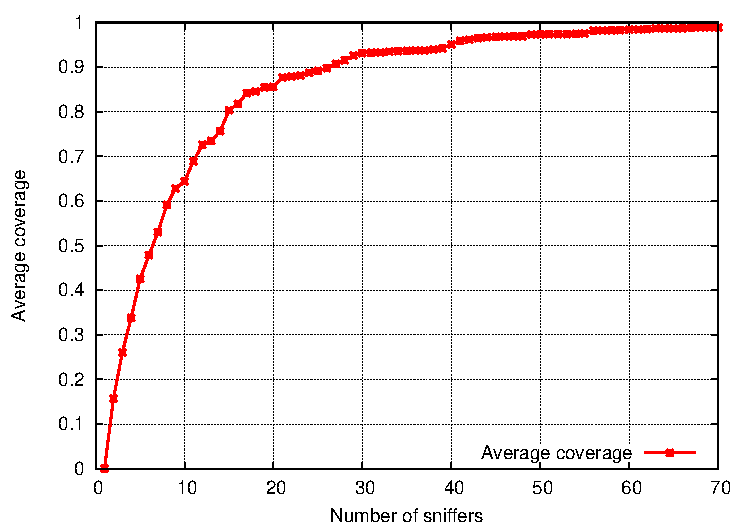
\includegraphics[width=0.6\hsize]{./resources/livenet-sensys07/figs/coverage/validation/coverage-motelab.pdf}
\end{center}
\caption{\small {\bf Sniffer coverage.}
{\em This plot shows the fraction of packets received by the sniffer
infrastructure as the number of sniffers is varied. Each point 
represents an average of 5~random configurations. Coverage of 
90\% is achieved with 27~sniffers.}}
\label{fig-sniffer-coverage}
\end{figure}

The next question is how many sniffers are required to achieve a
given {\em coverage} in our testbed. We define coverage as the
fraction of transmitted packets that are received by the LiveNet
infrastructure. There are 70~sniffer traces in total for this experiment.

To compute the coverage of a random set of $N$ traces, the most
thorough, yet computationally demanding, approach is to take all 
$N \choose 70$ subsets of traces, merge them, and
compute the resulting coverage. Instead, we choose five~random
permutations of the traces and successively merge them, adding
one trace at a time to the merge and computing the coverage. We then
take the average of the five~coverage values for each value of $N$. 
The results are shown in Figure~\ref{fig-sniffer-coverage}. 

As the figure shows, the first 17~traces yield the greatest contribution,
achieving a coverage of 84\%. After this, additional sniffers
result in diminishing returns. A coverage of 90\% is reached with
27~sniffers, and all 70~sniffers have a coverage of just under 99\%. 
Of course, these results are highly dependent on the physical extent
and placement of our testbed nodes. The testbed covers 3~floors of a
building spanning an area of $5226 \mathrm{m}^2$ (56,252~sq~ft). 
Assuming nodes are uniformly distributed in this area (which is not
the case), this suggests that approximately one sniffer per 
$193 \mathrm{m}^2$ (2077~sq~ft) would achieve a coverage of 90\%.
Keep in mind that sniffer locations were not planned to maximize coverage, 
and we are using the built-in antenna of the TMote Sky. High-gain
antennas and careful placement would likely achieve good coverage with
fewer nodes.


\subsection{Merge accuracy}


Next, we are interested in evaluating the accuracy of the merged
trace. As described earlier, our trace merging algorithm 
operates on fixed-length time windows and could lead to 
duplicate or reordered packets in the merged trace. 
Note that this can be avoided by reading in each of the
input traces into memory prior to merging, however, the memory
requirements of this approach are prohibitive. Performing a second
``self-merging'' pass on the trace can identify and correct duplicate
and reordered packets.

After merging all 70~source traces from the previous
experiment, we captured a total of 246,532~packets.
2920~packets are missing from the trace (coverage of 98.8\%). 
There are a total of 354~duplicate packets (0.14\%), 
and 13~out-of-order packets (0.005\%).
We feel confident that these error rates are low enough to rely on
the merged trace for higher-level analyses.

\subsection{Topology reconstruction}

\begin{figure}[t]
\begin{center}
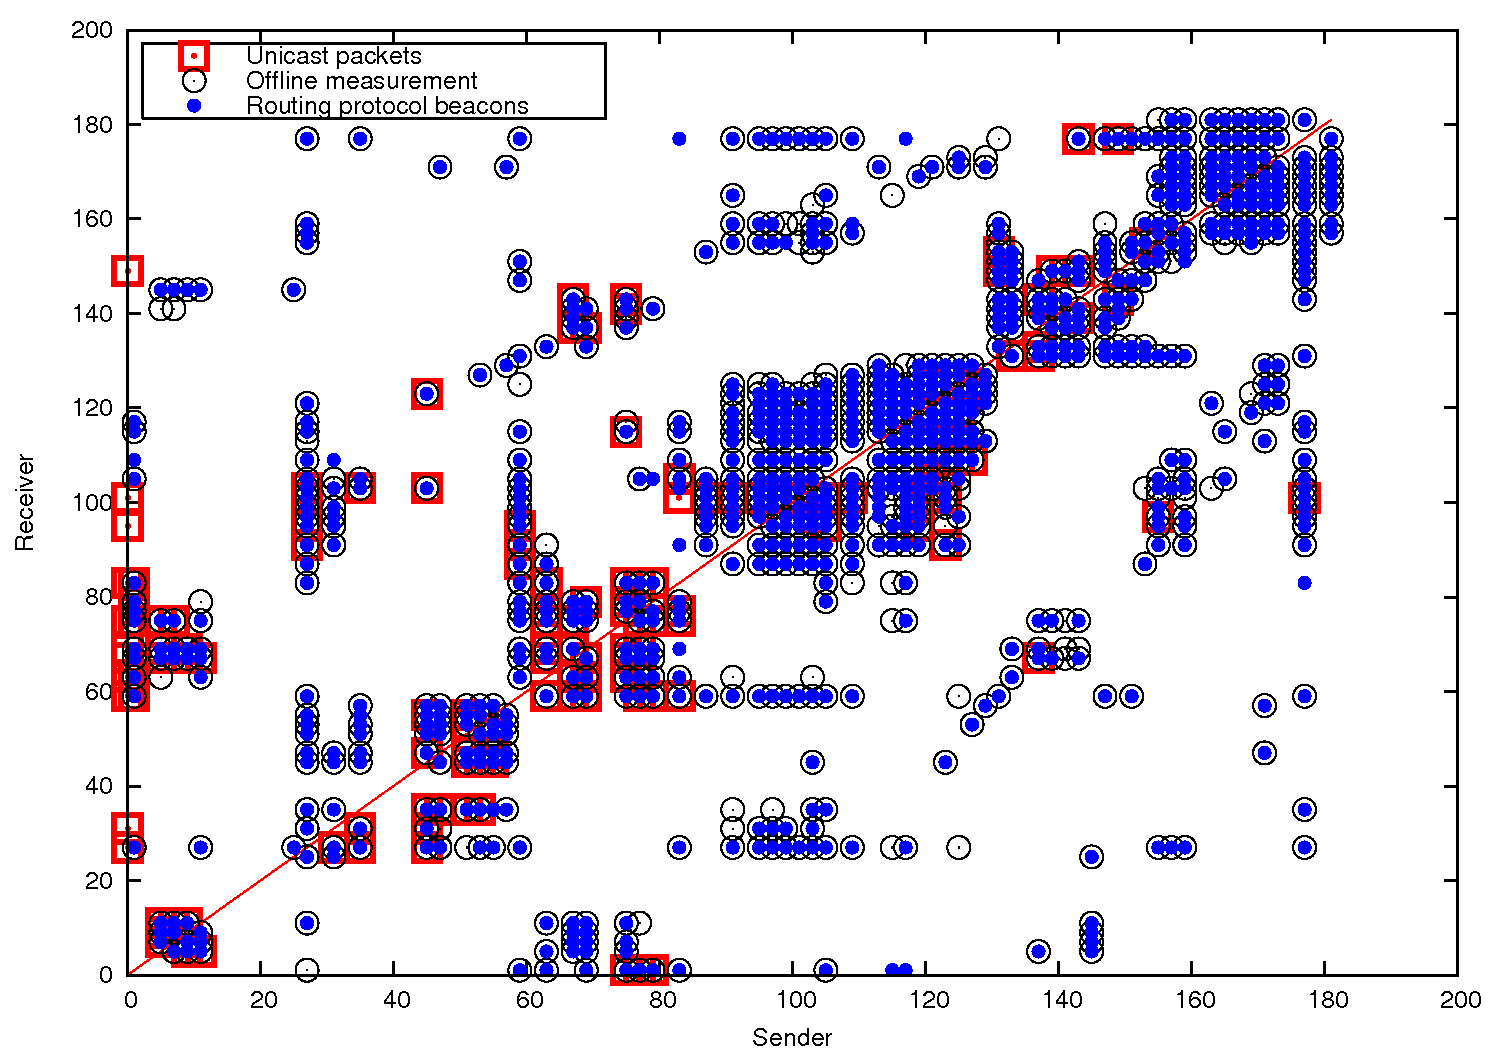
\includegraphics[width=0.6\hsize]{./resources/livenet-sensys07/figs/topology/validation/topology-compare.png}
\end{center}
\caption{\small {\bf Network topology reconstruction.}
{\em 
This figure shows the derived network topology from three
sources: (a) unicast transmissions along a spanning tree;
(b) extracted neighbor sets from routing protocol beacon messages;
and (c) an offline connectivity measurement. Each point represents a
single {\em (sender, receiver)} pair. As the data shows, there is
good correspondence between the beacon messages and offline
connectivity data, and very few links are discovered by observing
unicast transmissions alone.}}
\label{fig-topology-validation}
\end{figure}

\begin{figure}[t]
\begin{center}
\begin{small}
\begin{tabular}{|l|l||l|l|l|} \hline
                & {\em \# links} &  {\em Offline} & {\em Beacons}
		& {\em Unicasts} \\ \hline
{\em Offline} & 835 & -  & 777 (93\%) & 134 (16\%) \\ \hline
{\em Beacons}      & 799 & 777 (97\%) & -  & 134 (17\%) \\ \hline
{\em Unicasts}     & 146 & 134 (92\%) & 134 (92\%) & - \\ \hline
\end{tabular}
\end{small}
\end{center}
\caption{\small {\bf Comparison of topology data sources.}
{\em Each cell of this table shows the number of {\em matching} links
between each of three information sources: offline connectivity
measurement, routing protocol beacons, and unicast packets.}}
\label{fig-topology-comparison}
\end{figure}


We are interested in determining how well the LiveNet infrastructure
can recover the topology of our sensor network testbed. For this
experiment, we run the vital sign monitoring application on half of
the testbed nodes and sniffers on the other half. 
10 nodes were selected as patient sensors and
routed data along a spanning tree to a single sink node. There are
65~total nodes running the sensor application.

We use LiveNet to observe two
kinds of packets: {\em unicast transmissions} as packets traverse the
spanning tree, and periodic {\em neighbor table beacons} used by 
the application's routing protocol. Note that, in general, we expect
the neighbor table beacons to reveal many more links
than those traversed by unicast packets. 
We compare the LiveNet-derived topology to data obtained using an 
offline {\em connectivity measurement}, similar to SCALE~\cite{scale}, 
in which each node in turn transmits a series of packets, and all 
other nodes record the number of packets received from each source. 
We consider this data to be ``ground truth.'' The connectivity
measurement was performed immediately after we completed the LiveNet run.

Figure~\ref{fig-topology-validation} shows the complete set of links
determined using LiveNet and the offline connectivity measurement.
There are several interesting features of this graph. First, the
unicast packets reveal only a small number of links
(146~in this case). Second, network connectivity exhibits a fair
degree of asymmetry. Third, while there are a number of links not
observed by LiveNet, there are also links {\em only} seen in LiveNet
and not in the connectivity measurement.
Figure~\ref{fig-topology-comparison} gives a breakdown of the number
of links from each source of information. 22~links are seen only
in the routing beacon messages and not in the ``ground truth'' 
data set. We suspect this is due to poor link quality and the 
limited number of per-node
transmissions (10) used by the connectivity measurement. 

\subsection{Path inference}

\begin{figure}[t]
\begin{center}
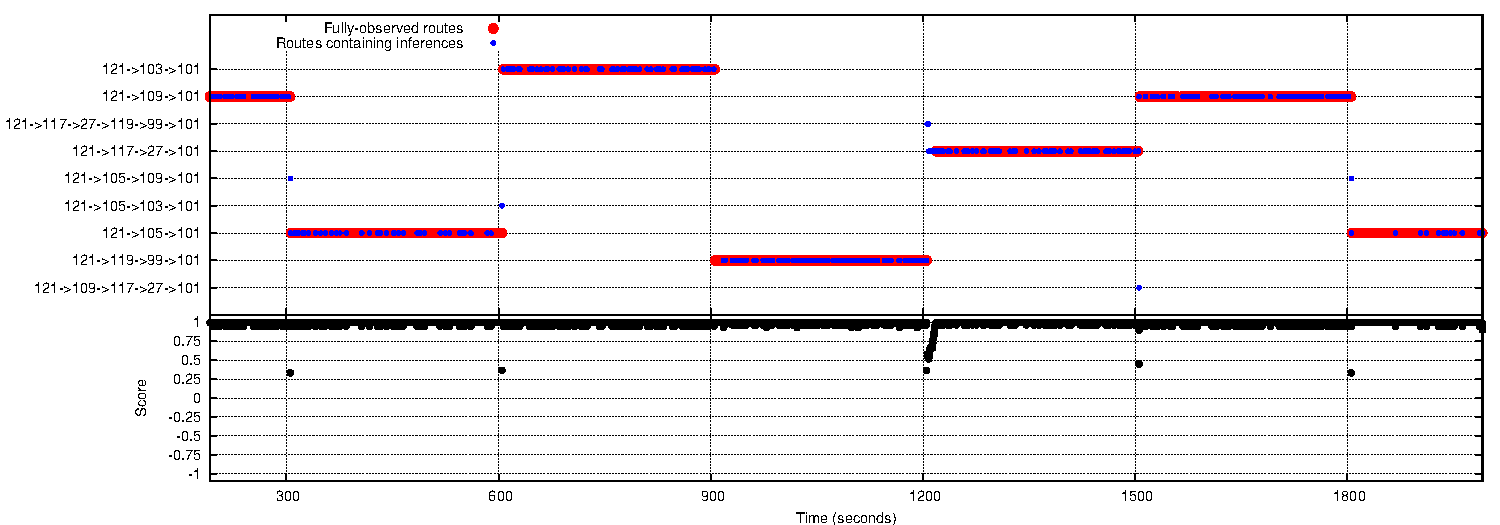
\includegraphics[width=0.9\hsize]{./resources/livenet-sensys07/figs/pathinference/motelab/path-motelab.pdf}
\end{center}
\caption{\small {\bf Path inference validation in the testbed.}
{\em This figure shows a plot of the inferred routing path for an
experiment in which a node is programmed to use a different routing
path every 5~minutes.
The top portion of the figure indicates the inferred path, and the
lower portion of the figure shows the mean $\Pi$ score over the
inferred path ($\Pi = 1$ indicates a complete observation of this path
at the given time).}}
\label{fig-path-validation}
\end{figure}

To test the path inference algorithm described in
Section~\ref{sec-livenet-path-inference}, we set up an experiment in which 
one node routes data to a given sink node over several multihop paths.
The node is programmed to automatically select a new route to the sink
every 5~minutes. Since we know the routing paths taken in advance, we
can compare the output of the path inference algorithm to ground
truth.

Figure~\ref{fig-path-validation} shows the results. The top portion
of the figure shows the routing path determined by the path inference
algorithm. Large points indicate routes that were fully observed by
the LiveNet infrastructure, while small points indicate routes
containing one or more inferred hops. The lower portion of the
figure shows the corresponding $\Pi$ score for the chosen path.

The paths inferred by our algorithm correspond to ground truth
in all but a few cases. For example, at times $t=300$, $600$, $1200$,
$1500$, and $1800$, there is an inferred path (with a relatively 
low $\Pi$ score) between two observed paths. This is because LiveNet
observes the path switch as it is taking place, so we briefly infer the
existence of an ``intermediate'' route. As expected the path switches
occur on 5~minute intervals.




\section{Design considerations and discussion}

LiveNet is designed to be entirely passive. Unlike other sensor network
debugging systems that require intrusive changes to the
application~\cite{sympathy,snms-ewsn05,rost2006memento,envirolog}, we chose to
not instrument the monitored application at all. Besides being general purpose, such
a design choice is motivated by the fact that we intend to use LiveNet to monitor
our CodeBlue deployment. Our CodeBlue prototype is based on MicaZ mote with
4KB of RAM. The CodeBlue implementation already uses almost all of the 4KB
available memory and has been already extensively tested on MoteLab. Adding
code for logging debugging information implies not only adding a simple
logging component but also re-writing parts of our application to reduce
memory usage and repeat a series of testing to make sure the software is
robust enough to run for our deployment duration. It would be too time
consuming and risky to add deployment monitoring code at such a late
development stage.

Also, we chose to not adopt SNIF~\cite{snif-demo-ewsn07} approach that
incorporates a Bluetooth backchannel to stream packet traces back to a base
station in real time. Trace merging in SNIF is therefore much simpler because
Bluetooth handles synchronization of the sniffer nodes already. In CodeBlue
scenario, we did not choose this approach because our application data rate is
much higher than that of SNIF's target applications. With high application
data rate, lively streaming packet traces back to a base station would not
only overwhelm the Bluetooth backchannel but also interfere with the
application packets, due to the use of the same 2.4GHz radio band. Also, the
capacity of the back channel limits the number of sniffers that can be
deployed with the network.  Moreover, being able to reliably collect packet
traces is of paramount importance to us because we would not have another
chance to organize another CodeBlue deployment. For this reason, we decided to
use laptops to store our packet traces instead of using a wireless backchannel or
storing data on the application nodes which may crash during the deployment.

Because of our application requirements, the design of LiveNet has to be
entirely passive and more reliable than other approaches proposed for wireless
sensor networks. Such requirements have also forced the later stages of LiveNet to
be more complex than in other systems. Merging of traces from unsynchronized
sniffers is one of the consequences from choosing to be entirely passive and
more robust. However, the resulted design of LiveNet makes it more scalable
and robust and therefore useful for a wider range of applications.

\section{Summary}
\label{sec-livenet-summary}

We have shown, through the development of LiveNet, that constructing an entirely
passive infrastructure for sensor network debugging and evaluation are quite
challenging. LiveNet is a toolkit that meets the requirements to
be entirely passive, scalable to a large number of sniffers, and include a set
of high level analyses.
To summarize, our contributions include the following:
\begin{itemize}
\item{Efficient and robust sniffer implementation}
\item{Algorithm for merging unsynchronized packet traces into one global trace}
\item{High level analyses for reconstructing the network dynamics, including
topology reconstruction, traffic breakdown, and a path inference algorithm}
\end{itemize}

As many other components of this dissertation research, a major goal of LiveNet is 
to be used for monitoring CodeBlue medical monitoring system. The requirements to be passive,
scalable and robust are determined by need of our CodeBlue deployment.
These requirements have led to a final design that is better than
other existing approaches in terms of robustness and scalability. We have
successfully deployed LiveNet with CodeBlue and are able to derive valuable
information by applying high level analyses proposed in this chapter to the
collected traces. Interesting results from the deployment are described in
the next chapter.

